\chapter{Interlude: Escape}

\begin{wrapfigure}{O}{\figwidth}
	\begin{center}
		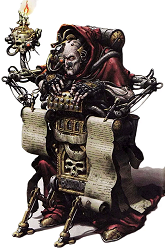
\includegraphics[width=\figwidth]{pics/20/1.png}
	\end{center}
\end{wrapfigure}

\greentext{>****** Security Level: Magenta ******}

\greentext{>Transcription Servitor Startup Sequence}

\greentext{>...}

\greentext{>...}

\greentext{>...}

\greentext{>Now is the time for all good men to come to the aid of The Emperor}

\greentext{>Planet: Joseph Haarlock Sucks at Cards}

\greentext{>Location: Precinct-House J1, Jack Hive, Meeting Room: Justice (277-A)}

\greentext{>Local Time: 21:15}

\greentext{>Date: [REDACTED]}


Governor-Marshal: 
In the name of the Emperor and the Pax Imperialis, I hereby call this fifteenth daily meeting of the Haarlockian Governing Council to order. 
Per the Regulations of Transitional Governments (Council), I will now call the roll and review the minutes of our last meeting.

Inquisitorial Observer: 
Not now man, everyone knows what they're here for, at least I hope you all do by now. 
Now let's get this started. 
Administratum, you first. 
Go. 


Administratum Representative: 
Ummm....

Governor-Marshal: 
Representing the Adeptus Ministorum, Priest Gregory Hammond. 
Representing the Adeptus Administratum, Sub-Prefect Laurence DuPont. 
Observing on behalf of the The Holy Orders of the Emperor's Inquisition, Inquisitor [REDACTED]. 
Representing the Haarlockian Noble houses-

\greentext{>* END PAGE 1 *}


\begin{wrapfigure}{O}{\figwidth}
	\begin{center}
		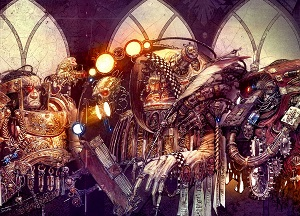
\includegraphics[width=\figwidth]{pics/20/2.png}
	\end{center}
\end{wrapfigure}

\greentext{>*PAGE 134*}


Ecclesiarchy Representative: 
-and finally we've begun recalling the Preachers we deployed to the lower hab blocks of Jack and Queen hive. 
We believe that the spiritual health of their lower classes is in acceptable order, but we have some concerns about-

Inquisitorial Observer: 
Yes yes, and your sending them to the middle and upper levels of Seven, as I suggested a week ago. 
Please inform that flatulent bag of augmetics and moral platitudes masquerading as this world's Deacon, that if he doesn't begin performing his duties with a little more alacrity I'll be forced to take personal control of your affairs. 
Or maybe I'll just second you all to the Orders Famulous, at least they know how to take a damn hint.

Ecclesiarchy Representative: 
I must humbly protest your-

Inquisitorial Observer: 
That's nice, anything else? 
No? 
Then your dismissed, all of you. 
No, don't look at him dammit, I said we're done here, go! 
Git! 
Off with you!

...

Governor-Marshal: 
Meeting Adjourned.

\greentext{>*END PAGE 134*}


\begin{wrapfigure}{O}{\figwidth}
	\begin{center}
		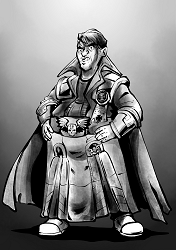
\includegraphics[width=\figwidth]{pics/20/3.png}
	\end{center}
\end{wrapfigure}

\greentext{>*PAGE 137*}


Inquisitorial Observer: 
Good show "Governor-Marshal", but if you could just dial that whole "The Law" thing back a little bit, that'd be great.

Governor-Marshal: 
Sir.

Inquisitorial Observer: 
Now where are we on the arrests? 
I've received confirmation that the Inquisitorial convoy will be arriving for them in three days, and I expect your men to have the entire collection ready.

Governor-Marshal: 
The last of the fugitives was apprehended this morning. 
We'll have shuttles ready to begin transferring them into your custody as soon as you're ready.

Inquisitorial Observer: 
My custody? 
Oh no, I'd be wasted on guard duty, and I've got plenty on my plate putting this whole mess of a planet back into working order. 
I shudder to think what you'd do without me. 
Don't worry, headquarters has sent several of their, shall we say, less intellectually inclined Inquisitors to handle the transportation of these traitors. 
I'm sure they'll be able to handle any problems, and I think I'll send my Interrogator along too... 
She's been having trouble staying "focused" lately; 
time for a change I think.

Governor-Marshal: 
Sir?

Inquisitorial Observer: 
Nevermind. 
Just be sure to have all your best Arbites on hand and briefed on the transfer procedures I sent over. 
Remember, the artifacts go first, then the Governor and his nobles, then the Secret Police, and THEN the varying Adepta traitors.

Governor-Marshal: 
And the Rogue Agents?

Inquisitorial Observer: 
What? 
Those idiots? 
This convoy is for the IMPORTANT prisoners, the whole point is to keep them as isolated from any outside support as possible. 


Governor-Marshal: 
So you've requested a seperate transfer ship then?

Inquisitorial Observer: 
For THEM? 
Of course not. 
While the Inquisition, not to mention me personally, will be more than happy to make an example, they themselves are completely unimportant. 
Just send them over on the next Arbite prison ship you've got going that way.

\greentext{>*END PAGE 137*}


\begin{wrapfigure}{O}{\figwidth}
	\begin{center}
		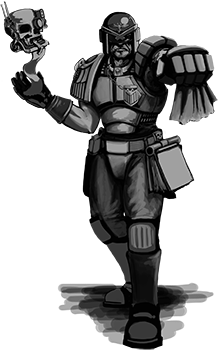
\includegraphics[width=\figwidth]{pics/20/4.png}
	\end{center}
\end{wrapfigure}

\greentext{>*PAGE 138*}


Governor-Marshal: 
Adeptus Arbite vessels are not "prison ships". 
They are the Fist of the Emperor's Justice, Enforcers of the Pax Imperialis, The Longest Arm of The-

Inquisitorial Observer: 
Yes, yes, I get the picture, but they ARE Imperial Vessels: 
they surely have a brig, or at the very least a closet or laundry room where you dump drunken crew. 
Chuck the idiots in there.

Governor-Marshal: 
You are instructing me to transport a rogue team highly trained Inquisitorial agents to their trial... 
In. 
A. 
Laundry room.

Inquisitorial Observer: 
Oh come on. 
They're "highly trained Inquisitorial agents" in the same sense you were a traffic officer, just because someone with a low sense of humor declared them such doesn't make it true. 
And in any case, they'll be on an entire ship full of Arbites! 
Not even the most brain-damaged, slow-witted, incompetent, meathead of an officer would let themselves... 
um, be taken by, um...

Governor-Marshal:...

Inquisitorial Observer: 
Well, I mean, actually- 

Governor-Marshal: 
Very well, I'll see to their delivery to Inquisitorial Headquarters personally. 
My second in command will fill in-

Inquisitorial Observer: 
No!

Governor-Marshal:...

Inquisitorial Observer: 
I, uh, need you here. 
To keep things running, maintain the Rule of Law on this dangerously criminal world, and all that stuff.

Governor-Marshal:...

Inquisitorial Observer: 
Look, just ship them off and don't worry about it. 
That's a direct order.

Governor-Marshal:...Sir.

Inquisitorial Observer: 
Good. 
That's settled then. 
Just let me know when your ship arrives, should have some of the mundane evidence cataloged and ready for transport by then, and possibly report on-

\greentext{>*END PAGE 138*}


\begin{wrapfigure}{O}{\figwidth}
	\begin{center}
		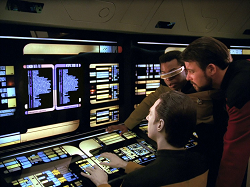
\includegraphics[width=\figwidth]{pics/20/5.png}
	\end{center}
\end{wrapfigure}

\greentext{>Watch Log, The Unflinching Adherence}

\greentext{>Current Anchorage: Jack Station, Joseph Haarlock Sucks at Cards}

\greentext{>Current Shift: 1}

\greentext{>Officer of the Deck: First Officer Mills}

\greentext{>Timestamp: [CORRUPTED]}

\greentext{>New Section Begins: 0615-0620.log}


First Officer: 
He wants us to put them WHERE? 
Doesn't he know we have a brig?

Communications Officer: 
Yes, I told him, he said the Inquisitor requested it specifically.

First Officer: 
The Inquisitor? 
These are Inquisitorial prisoners?

Communications Officer: 
He, um, didn't say. 
Just that they "weren't important", and that their crimes were included in the official transfer request. 
I have it here.

First Officer: 
These are parking violations... 
Are you SURE he was the Governor-Marshal? 


Communications Officer: 
Yes, definitely. 
Very, very definitely.

First Officer: 
... 
none of this makes any sense.

Communications Officer: 
I told him that sir. 
He just said it wasn't our job to understand The Law, just enforce it.

First Officer: 
Hmmm, he's right about that at least... 
Who the hell did these guys piss off to get themselves shipped to Inquisitorial Headquarters for a bunch of unpaid parking tickets?

Communications Officer: 
The Inquisition?

First Officer: 
Well obviously, the poor dumb bastards. 
Get this filed away to the Quartermaster's office along with the shipping request, and inform the Head Medicae that she's getting a new patient. 
Oh, and send a copy to the Head Proctor as well; 
at least this means we can switch a few of his trainees from janitorial to guard duty, he'll like that. 
Now, PLEASE tell me the rest of the overnight communiques were more sensible.

\begin{wrapfigure}{O}{\figwidth}
	\begin{center}
		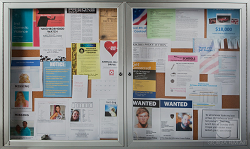
\includegraphics[width=\figwidth]{pics/20/6.png}
	\end{center}
\end{wrapfigure}

\greentext{>**********ANNOUNCEMENTS**********}

\greentext{>All Hands Notice: Laundry Room B}

Until further notice, Laundry Room B is considered a restricted area off limits to ship crew and to be kept under guard at all times. 
Laundry deliveries and pickups will continue as scheduled via the starboard entrance. 
Contact the Training Office with any issues relating to this change.

\greentext{>ALL HANDS NOTICE: TECH-HERESY}

THE MODIFICATION OF SHIP SYSTEMS BY THE UNORDAINED IS AN ABOMINATION IN THE PHOTORECEPTORS OF THE OMNISSIAH. 
ACTS OF TECH-HERESY WILL BE PUNISHED, YOU HAVE BEEN WARNED.

\greentext{>All Hands Notice: Laundry Changes}

Laundry Room B is to remain sealed to ALL personnel pending Mechanicus inspection. 
Repairs on the surrounding rooms and corridors are scheduled for completion within three days. 
Until further notice, Laundry Room A is considered a restricted area off limits to NON-ESSENTIAL ship crew and to be kept under guard at all times. 
Laundry deliveries and pickups will continue as scheduled via the port entrance, including all laundry originally routed to Room B. 
Contact the Training Office with any issues relating to this change.

\greentext{>All Hands Notice: Laundry Schedule}

Laundry will be processed in the order it is collected and delivered. 
Priority will NOT be given to ANYONE.

\greentext{>All Hands Notice: Fraternization with Prisoners}

All Arbites and ship crew are reminded that personal and commercial interactions with prisoners, including those confined to locations other than the brig, is forbidden and will be punished if discovered. 


\greentext{>All Hands Notice: Reminder, Regulations on Gambling}

All Arbites are advised that while the Pax Imperialis does not concern itself with gambling, under Arbite Naval Regulations all games of chance are strictly forbidden. 
Crew are strongly encouraged to follow this example a well.

\begin{wrapfigure}{O}{\figwidth}
	\begin{center}
		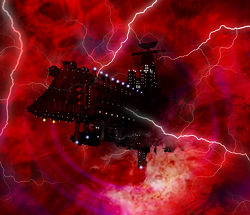
\includegraphics[width=\figwidth]{pics/20/7.png}
	\end{center}
\end{wrapfigure}

\greentext{>All Hands Notice: Lost Equipment}

All hands are reminded that, per Arbite Naval Regulation 39M-1025-J any equipment assigned to them by the Quartermaster's office is THEIR responsibility and its misplacement is considered a class-3 infraction.

\greentext{>All Hands Notice: Identification Badge}

Any Arbite or crew to come across an unattended Identification Badge is to immediately deliver it to the Head Intelligencer's office.

\greentext{>Lost and Found}

A Lost and Found office has been established adjacent to Laundry Room A (some fees may apply)
-Head Intelligencer Clouseau

\greentext{>All Hands Notice: Reminder, Firing Range Rules}

ALL weapons, ammunition, and wargear checked out for training purposes must be either expended or returned by end of shift. 
Any Arbite who fails to adhere to these rules will be banned from the range.

\greentext{>All Hands Notice: Firing Range Restrictions}

The following items are no longer available at the firing range until further notice: 

*Anti-personnel mines
*Breaching Charges
*Demolition Charges
*Frag, Krak, and Flash Grenades
These restrictions will be lifted following the next resupply.

\greentext{>All Hands Notice: Warp Storm}

The Navigator has identified an unexpected Warp Storm obstructing our course. 
All Arbites, including trainees, are to assume their counter-boarding stations until such time as the Navigator gives the all clear. 
The forward and aft chapels will be holding continuous services for the duration.

\greentext{>All Hands Notice: Conspicuous Valor in the Face of the Unholy}

Trainees Mullroy and Murtogg are hereby promoted to full Trooper in recognition of their miraculous, completely unassisted defense of the starboard section of Deck 3 during yesterday's warp-incursion.

\greentext{>Medical Work Release Program}

Due to the recent influx of wounded, select medically-trained prisoners have been granted ship access between Laundry Room A and the Medbay under supervision of Troopers Mullroy and Murtogg.
-Head Intelligencer Clouseau

\begin{wrapfigure}{O}{\figwidth}
	\begin{center}
		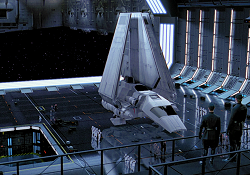
\includegraphics[width=\figwidth]{pics/20/8.png}
	\end{center}
\end{wrapfigure}

Terrance Dockbosson, fifth of his name and Shift-3 Dockboss of Small-Craft Bay 12, watched approvingly as his team moved to receive the last incoming shuttle of the shift. 
His appreciative nodding and thoughts of the meal waiting in his cabin were interrupted by the opening of one of the Bay's personnel doors and the arrival of two fully armored Arbites. 
Knowing a snap inspection when he saw one, Terrance regretfully bid all thoughts of a hot soya dinner goodbye and moved to greet the taller of the pair, who looked to be a full Investigator instead of the usual grunts that drew the duty. 
He was surprised, albeit pleasantly, when the helmeted Investigator waved off his proffered manifest, and merely ordered him to "Gas it back up, and then take an early break, we'll handle the rest." 

Terrance rounded up his team and directed the Investigator towards the bay's master control altar, which the taller Arbite was unexpectedly interested in. 
As they made their way towards the exit, the youngest member of his team, paused and asked whether it was really okay to leave their post before the end of shift. 
The dockboss just paused and directed the boy's attention to where the shorter Arbite was waving a stack of official documents in the face of an annoyed shuttle pilot, who batted them aside and asked "Aren't you a little short for an Arbite?"

The Arbite shrugged "Aren't you a lil moufy for a deliveryman what wants to get a proper tip an' not 'ave 'is knees broke?" As the pilot, who was evidently unfamiliar with Arbites and their penchant for literalness, puffed up with indignation and began to respond, Terrance clapped the boy on the shoulder and steered him out the exit. 
The door shut behind them on a bellow of "I'm not a damn deliveryman you lit- MY KNEE!"

Decades later, Judge-Captain Terrance Dockbosson the Sixth, fondly recalled that as the day he decided to abandon several generations of family tradition and enlist in the Arbites.

\begin{wrapfigure}{O}{\figwidth}
	\begin{center}
		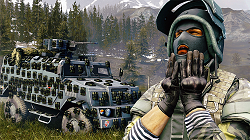
\includegraphics[width=\figwidth]{pics/20/9.png}
	\end{center}
\end{wrapfigure}

Nubby had just finished cramming the annoyingly loud pilot into a handy shipping container, without any help from Tink mind you, when one of the bay's doors opened to admit two more "Arbites" pushing a loaded pallet and wheelchair respectively.

"Why's the shuttle still closed Tink?" asked the wheelchair-pushing Arbite. 
"We've got a bit of a time limit here you know."

Up at the control altar, Tink jabbed a few more buttons before throwing his arms up in the air "What the hell do you want me to do about it smartass? 
This thing just controls the doors and maglocks! 
Go ask Nubby, he's the one who was too busy arguing with the pilot to notice it closing."

"I fought 'e 'ad a key or somefin! 
What sort of idiot locks 'imself out of his own damn shuttle, dat's what I wanna know."

Doc groaned and rubbed his oversized helmet as the pair started arguing. 
He looked to his wheelchair's occupant for some sort of direction, but given the amount of anesthetics and painkillers Sarge was currently on, all he got was a few spit bubbles and a snore. 
Twitch watched the pair for a second in case an order of some sort was forthcoming, and then shrugged, popped open one of the crates on his pallet and pulled out a breaching charge. 
He'd already started adhering the explosive to the shuttle's airlock before the other guardsmen noticed what he was doing and shouted at him to stop. 


\begin{wrapfigure}{O}{\figwidth}
	\begin{center}
		
\includegraphics[width=\figwidth]{pics/20/10.png}
	\end{center}
\end{wrapfigure}

The demolitions trooper turned to see why everyone was so upset about him sticking explosives to their getaway vehicle. 
Behind him the airlock door slid open, briefly sticking on the charge before scraping it off, to reveal three figures. 


The robed, dataslate-holding man on the left paused as his foot landed in something sticky, looked down and froze. 
The carapace-armored and helmeted Sister of Battle on the right of the group froze as well, staring blankly at the assorted "Arbites" at the bottom of the ramp. 
The third figure, the one with the Ordos Xenos Inquisitorial Rosette on chest, didn't freeze. 


"Now if one of you could be so kind as to explain what in the Emperor's name do you think you're doing here, I might just be willing to... 
Interrogator Sargent?"

Nubby, Tink, and Twitch all made choking noises, Doc however popped his visor up, and looked Inquisitor Oak straight in the eye. 
"Escaping?"

The Inquisitor paused, began to speak, paused again, and then exploded. 
"Oh, you've GOT to be kidding me. 
NOW, you're doing this NOW!?" All four guardsmen took a step backwards. 
"Do you have ANY idea how hard this is going to make-" the Inquisitor abruptly broke off his rant and deflated. 
"No, of course you don't, you didn't "need to know" did you?"

"You don't mean-" began Tink, only be cut off as the dataslate wielding Interrogator announced "Ten minutes sir."

Oak winced. 
"No time, I'll explain later, I promise you, but if I'm going to salvage this I need all of you to get back to your cells RIGHT NOW."

\begin{wrapfigure}{O}{\figwidth}
	\begin{center}
		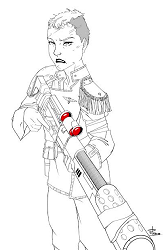
\includegraphics[width=\figwidth]{pics/20/11.png}
	\end{center}
\end{wrapfigure}
Twitch looked to Nubby, who looked to Tink, who looked to Doc, who vainly looked down at Sarge for a second before accepting that the buck had well and truly stopped. 
Oak, seeing the hesitation and interpreting it as something more than agonized dithering let out an annoyed groan, and turned to the Sister of Battle at his side. 
"Would you PLEASE do something about this?" 

Amelia Delorisista Amanita Trigestrata Zeldana Malifee von Humpeding shrugged, pulled off her stupid helmet, and announced "Come on you idiots, let's go. 
Back to your cells." She jogged down the ramp, past a slackjawed Twitch and Nubby, and without pausing grabbed the wheelchair from Doc. 
"Double time soldiers, THAT'S AN ORDER GUARDSMEN! 
Right Sarge?" 

The snoring noncom jerked in his seat and slurred "habs n order guarshem", before slumping over again. 


Twitch, Nubby, and Doc shared a look and a shrug, and then filed after the pair. 
Up at the control altar, Tink grumpily undid the door control overrides he'd just implemented, and with a mutter of "worst escape attempt ever..." fell in at the end of the line.

\begin{wrapfigure}{O}{\figwidth}
	\begin{center}
		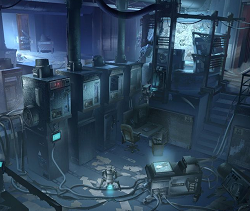
\includegraphics[width=\figwidth]{pics/20/12a.png}
	\end{center}
\end{wrapfigure}

Aimy leaned back in her chair and kicked her black-and-red carapace-armored feet up on the large table in the middle of the laundry-brig. 
Across from her, Nubby paused from helping Twitch unload their pallet full of crates to open one of them and pull out a double-handful of bottles. 
The markswoman snagged the one that was slid her way, and sipped at it as she eyed the familiar clutter of boxes, barricades, and the occasional loop of razorwire littering the room. 


Admittedly all the piles of laundry and the large machines lining the walls were a bit out of place. 
Not to mention the haphazard network of pipes, wires, and chutes linking everything to some sort of giant rats nest in the far corner of the room where Tink was swearing at something or other. 
Over all it was very homey, though she did wonder where the sandbags had come from.

"Nice digs, expected something a bit more, you know, prison-y."

Tink poked his head from behind the kludged-together control-altar he was abusing. 
"Yeah, guess the Arbites are too incompetent to do their own laundry or something and wanted some expert help. 
Nice hair by the way, looks like she nearly got it all one color this time, and only a moderate amount of facial scarring too!"

Tink flinched as Aimy drew her bottle back for a throw, but relaxed as she decided there were better uses for the first beer she'd even SEEN in over a month.

"Yeah, well, Doc's girl does good work doesn't she?" The markswoman turned her head towards the curtain that had been hung around one of the bunks at the far end of the room, and raised her voice slightly, "Even if 'My dearest Val-entine' gets tad on the bitchy side without her boy-toy around to play doctor."

There was a strangled sound of protest from the little makeshift operating theatre, followed by crashing clatter and a series of curses. 
Nubby and Tink both snickered; 
Twitch went to inspect the disturbance for signs of hostile activity. 



\begin{wrapfigure}{O}{\figwidth}
	\begin{center}
		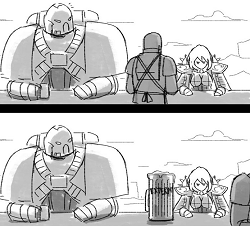
\includegraphics[width=\figwidth]{pics/20/13.png}
	\end{center}
\end{wrapfigure}

Aimy smirked and sipped her drink before continuing. 
"Seriously though, shoulda heard what she said to Oak when he turned up out of nowhere wanting to haul me off. 
If the Adept wasn't there to talk her down she'd have probably given him a round of involuntary treatment. 
The old smoothtalker brought her around though," she paused and tapped her cartoonishly oversized "breast plate", "even convinced her to loan me her combat gear for this whole Sister disguise thing."

"Ah..." Nubby made a face, "You sure it's jus' a disguise, cause I got somefin like tweny crates of bolter ammo round here somewhere... 
not sure why I even lets 'em pay wif dat stuff anymore."

"What was the disguise even for anyway?" asked Tink, "Did Oak need someone to inspect a Soritatas Convent for signs of 'deviant practices' and figured you'd know where to look?"

Aimy flipped a single finger in Tink's direction and then shrugged, "No idea, he's a tight lipped fucker aint he? 
And I swear that Interrogator of his hasn't spent more than ten minutes off that dataslate since I met them. 
All I know is they showed up in the medbay with the Adept and said you guys needed my help, and that I'd have to disguise myself as," the markswoman adopted a slightly creaky lecturing tone "Literally anything that isn't a guardswoman, if you can manage that."

Aimy paused to sip her drink, "Didn't tell me a single fucking thing about what was actually going on, just that you guys had done better than expected on your mission, and had 'infiltrated' an Arbite vessel on its way to Inquisitorial Headquarters. 
I asked he was sure he hadn't meant 'arrested', and Oak said the agent he'd sent to contact you hadn't been able to confirm anything, which is why we were all going."


\begin{wrapfigure}{O}{\figwidth}
	\begin{center}
		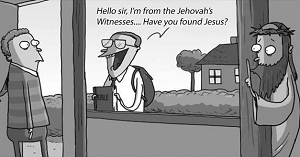
\includegraphics[width=\figwidth]{pics/20/14.png}
	\end{center}
\end{wrapfigure}

Twitch abruptly poked his head out from the operating theatre, "Agent? 
What Agent? 
How was he supposed to contact us, what was his call sign?"

"How the hell should I know?" Aimy shrugged again, " I gathered it was some guy you knew, one of you old Interrogators I think?"

Twitch paused, leaned back behind the curtain to ask Doc something, and then started swearing. 
Nubby and Tink both stared in confusion for a few seconds before the shorter trooper abruptly snapped his fingers 'Ohhhhhh, I fought I recognized dat guy from somewhere! 
Shoulda said 'e was 'ere from Oak. 
Burstin in all unannounced, shoutin bout 'ow we 'ad to 'ide 'im fore the Arbites got 'ere didn' quite convey the message  "

Aimy raised an eyebrow "So what happened to him?"

"See dat blast mark over dere?" Nubby gestured towards a stained section of deckplate only a few steps from the door. 
"Twitch DID tell 'im to stop. 
Least we got the rest of em disarmed 'fore the Arbites showed up to grab 'im. 
"

Tink chimed in, "And Doc said the head medicae got his leg back on before they hauled him off to the brig."


\begin{wrapfigure}{O}{\figwidth}
	\begin{center}
		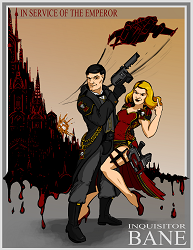
\includegraphics[width=\figwidth]{pics/20/15.png}
	\end{center}
\end{wrapfigure}

There was a lull in the conversation, in which a faint metallic clicking could he be heard from behind the curtain. 
Aimy shook her head and took another sip, "So, speaking of Doc, and whatever half-assed medical procedure he's conducting back there-" her casual tone became a bit forced "Would anyone care to explain why the fuck Sarge is riding around in a wheelchair in nothing but a hospital gown, high as a kite and minus one hand?"

Nubby flinched and looked at Tink, who was suddenly completely engrossed in his master laundry-control-unit. 
The ugly little trooper sighed, picked his nose thoughtfully.

"You, uh, 'member Bane Johns?"

"No?" Aimy paused, "Wait, you mean Twitch's Vampire Ork guy?" There was a triumphant shout from the far side of curtain. 
"You mean he was real? 
And wasn't he hauled off to some sort of prison, just like That Bitch was?"

"Yeah, umm, about dat. 
So no shit, there we were..."


\begin{wrapfigure}{O}{\figwidth}
	\begin{center}
		
\includegraphics[width=\figwidth]{pics/20/16.png}
	\end{center}
\end{wrapfigure}

Inquisitor Quercus, or Oak as his numerous underlings insisted on calling him, took a second to collect this thoughts before keying open the warning-covered laundry room door. 
The meeting with the Judge-Captain had gone quite well, the man and his First Officer had proved to be unexpectedly aware of the storm clouds gather on the horizon, and Oak had always held with the old Inquisitorial adage: 
"A Little Truth Goes a Long Way". 
He made a note to do something for extra for their careers, and maybe see if they had any promising new recruits coming up through the ranks. 
Assuming he survived the storm himself, of course.

Oak's trip down to the evidence lockers to review Inquisitor Sciscitat's in-depth report had been a less enjoyable experience. 
He couldn't deny that the mission had been successful, beyond all reasonable expectations really, given the situation. 
The man's initiative was commendable, and his plan for the next stage was good as well, if not quite as brilliant as his astropathic message had suggested... 
But all that aside, how mind-bogglingly close EVERYTHING had come to total failure, and for such stupid reasons, shook him to his core. 
It was beyond Oak's understanding how someone with such an amazing analytical mind could be so petty, insufferable, and incapable of seeing the results of their own actions. 


He'd left his Interrogator to sift the rest of Sciscitat's drivel for the pertinent details; 
right now he needed to go have a chat with some guardsmen before they did anything else to destabilize the balance of the sector.


\begin{wrapfigure}{O}{\figwidth}
	\begin{center}
		
\includegraphics[width=\figwidth]{pics/20/17.png}
	\end{center}
\end{wrapfigure}

"-but turns out nobody told that crazy fucking cogboy about the whole "door" thing during warp turbulence, so you remember those squigs he was keeping to see if they could be turned back into genestealers? 
Well, the good news is Hydroponics Bay 3 no longer has a mutant krootoid problem... 
Oh, and Jim wanted me to let you know that some sort of smelly shadow monsters nicked all that stuff you had stashed under deck seven and disappeared."

"THOSE UNGRATEFUL BASTARDS!"

"So over all, pretty normal until Oak showed up and had this big secret meeting with the Adepts and the mad magos-"

Inquisitor Quercus cleared his throat. 
Aimy flinched and scattered the better part of a dozen bottles as she tried, and failed, to stop herself from tilting over backwards. 
The two guardsmen sitting on either side of her scrambled to shove their own collections of bottles under the table. 
The exhausted medic slumped a little farther up didn't bother, neither did the trooper who'd watched Oak enter, preferring to remain completely focused on the Inquisitor's movements while fingering something held just under the table. 
Oak carefully moved his hands a little farther from his weapons, and directed his attention to the last guardsman, the one sitting at the end of the table and still wearing a hospital gown. 


Interrogator Sargent rose slightly-unsteadily to his feet and began to salute, only to pause as he remembered his one medically-approved drink in his hand and switched his left. 
There was a metallic thunk as the shiny new augmetic hand rebounded off his forehead with the force of a small hammer. 
He swayed for a second, attempting to maintain eye-contact with Oak, and them abruptly sat back down. 
From her position on the floor, Aimy fumbled through the bottled around her before settling on an unopened one and raising it in the air above her. 
"Hi boss! 
They got beer! 
Want one?"

Oak surveyed the room for a few seconds longer, and then sighed. 
"Yes. 
Yes I really think I do."


\begin{wrapfigure}{O}{\figwidth}
	\begin{center}
		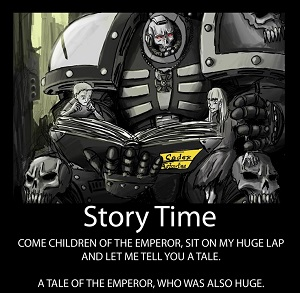
\includegraphics[width=\figwidth]{pics/20/18.png}
	\end{center}
\end{wrapfigure}

\greentext{>"I'm going to tell you a story."}

\greentext{>"A long time ago there was an Interrogator, who served an Inquisitor in the Ordos Hereticus. For several years they pursued a heretical cult whose influence was so subtle and mysterious, that even their Inquisitorial comrades questioned its existence."}

\greentext{>"In the end they finally tracked the cult to an Imperial Schola Progenium. They purged the Schola, but before their deaths the heretics managed to summon a powerful daemon and bind it in the body of the Schola's high Abbot, who killed all but a handful of the Inquisitor's team before he was destroyed. Following this bitter victory, the Inquisitor decided to retire to a administrative role within his Ordos and the Interrogator was promoted to full Inquisitor, but at his master's insistence, he took up service in a separate branch of the Inquisition."}

\greentext{>"Several years later the junior Inquisitor encountered two rumors, one of a new theory for the training of Inquisitorial agents, and the other of a new Inquisitorial power bloc which welcomed more radical members into its ranks. Something about these rumors struck him as familiar, so despite both these things being outside the purview of a junior Ordos Xenos Inquisitor, he followed them to their source, which turned out to be his old master. He confronted his master, but not alone, and not peacefully."}

\greentext{>"Five Inquisitors died that day, including the master, who fought with a completely unexpected strength and ferocity. The junior Inquisitor later believed he was a daemonhost, and claimed he recognized from the cult's lair. The senior Ordos Hereticus Inquisitor who led the investigation disagreed. Decades later, a proposal for the foundation of an Inquisitorial school was put forth by the very same woman, the no-longer-very-junior Inquisitor found this to be suspicious and investigated, with prejudice. The results were similar. "}


\begin{wrapfigure}{O}{\figwidth}
	\begin{center}
		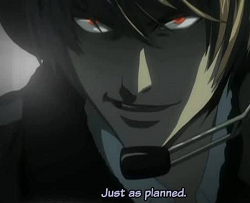
\includegraphics[width=\figwidth]{pics/20/19.png}
	\end{center}
\end{wrapfigure}

\greentext{>"Six times, six damn times I've killed that thing, and every time it comes back in the body of one of my comrades. I've tried every banishment known to the Inquisition, at least all those the Ordos Malleus will share with me, and it just keeps coming back, even the time we just burned the entire planet from orbit. Eventually it got just as tired of dying as I was of it coming back though, it decided to just wait me out, laying low and pulling at strings from somewhere inside Inquisitorial headquarters, still trying to get that heretical school of its founded. So I did the only thing I could think of, I stole the damn thing's idea out from under it."}

\greentext{>"And now here I am, glorified kindergarten teacher to a never ending stream of psychopaths, incompetents, and power seekers whose own Inquisitors couldn't be bothered to properly mentor them. Not where I saw myself when I was a starry eyed young adept, but at least it gives me some influence and I use it as best I can to foil that damn thing's plans."}

\greentext{>"For the least century and a half we've been in this stalemate, dancing around and keeping each other cut down to size. The damn thing has been gaining on me though, slowly picking off my supporters and alienating me from the rest of the Inquisition, but I'm not done yet, and this time I have a way to end things once and for all. It must think so too, otherwise it wouldn't have launched its attack so prematurely. It and its Conspiracy may have branded me a Rogue and neutralized most of my teams and allies, but it exposed itself in the process, and where it really, truly mattered, it completely botched things."}

\greentext{>"Which brings me to you."}


\begin{wrapfigure}{O}{\figwidth}
	\begin{center}
		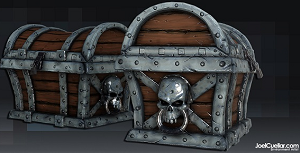
\includegraphics[width=\figwidth]{pics/20/20.png}
	\end{center}
\end{wrapfigure}

\greentext{>"With your help Inquisitor Scicitat secured a collection of heretical artifacts which had been stolen, re-stolen, and then re-re-stolen. Those artifacts, along with Sciscitat's official report and every heretic on that benighted world, were put on an official Inquisitorial convoy guarded by every single suspected traitor, closet radical, and power-hungry idiot both the Conspiracy and my remaining allies at Sector Headquarters could find. Putting all the bad eggs in one basket, as they say. I beleive this vessel passed through what was left of them just over a week ago."}

\greentext{>"The boxes which had held those artifacts on the other hand, are sitting in this ship's hold, being used to transport your personal effects and other assorted mundane evidence to the Sector's Inquisitorial headquarters. Or they would be, if you weren't currently using them to store a mixture of high explosives and alcoholic beverages, which you seemingly intended to take with you as you deserted off to Emperor knows where. I am, for perhaps the first time in Inquisitorial history, going to assume that you weren't doing this out of some heretical desire to undermine the fabric of the Imperium, and just "didn't need to know" that the entire reason you are on this ship is to smuggle those boxes into Inquisitorial Headquarters, where I intend to use them to banish this daemon once and for all."}


\begin{wrapfigure}{O}{\figwidth}
	\begin{center}
		
\includegraphics[width=\figwidth]{pics/20/21.png}
	\end{center}
\end{wrapfigure}

Sarge blinked at the Inquisitor for a second, and then shot a look at Nubby, who seemed caught between incredulity and defensiveness. 
Doc put a hand over his mouth before one could win out. 
Oak leaned across the table towards Sarge. 
"Now that you DO know though, what I need you to do is put those boxes back exactly where they were, complete with their contents assuming you haven't hocked them for booze money or something similarly ridiculous."

Nubby made a sputtering sound from behind Doc's hand; 
Oak ignored it, "Then, I need you to promise to stay put and allow yourselves to be transported to Inquisitorial Headquarters for your trial."

Tink broke his uncharacteristically long silence, "Are you nuts? 
They'll shoot us for heresy!"

Oak rolled his eyes at him, "No, they won't." He held three fingers up in Tink's direction and ticked one down, "First of all, despite all the impressive, and quite frankly ridiculous, things you've managed to accomplish in your short Inquisitorial career, the Conspiracy does not consider you an Important. 
Presumably because of the two agents who actually knew you long enough to get past your rather unique first impression, one was executed by my own agent before he could send a report, and the other fervently argued that it was all dumb luck right up until the point you incinerated her."


\begin{wrapfigure}{O}{\figwidth}
	\begin{center}
		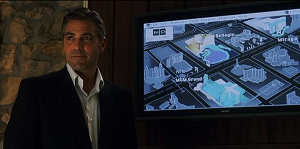
\includegraphics[width=\figwidth]{pics/20/22.png}
	\end{center}
\end{wrapfigure}

The Inquisitor lowered another finger, "Secondly, the charge is not Heresy, or Impersonating an Inquisitor or Astropath-icide for that matter. 
It's Assisting a Rogue Inquisitor, and unless you are considered particularly dangerous or important, the punishment for that is imprisonment in stasis until said Inquisitor's trial. 
After which you're released into their custody pending official review of your actions" he paused for a second "or if they're guilty, summarily executed via plasma incineration."

Tink made a strangled sound, "How is that any bet-"

Oak, cut him off, "And finally, I have arranged with my remaining agents at Inquisitorial Headquarters to have your sentence commuted. 
You will instead be assigned to considerably lower-security holding facility, which just so happens to be adjacent to the mundane evidence storage warehouse, putting you in perfect position to infiltrate it and move the Boxes from the storage unit assigned to your case, to the one assigned to mine."


\begin{wrapfigure}{O}{\figwidth}
	\begin{center}
		
\includegraphics[width=\figwidth]{pics/20/23.png}
	\end{center}
\end{wrapfigure}

As the Inquisitor leaned back into his chair and tented his fingers in front of him, Tink, Nubby, and slightly-slurring Aimy all burst into objections. 
Sarge ignored them and looked to Doc, who scratched his head for a second then shrugged. 
Across the table, Twitch raised the detonator in his hand ever so slightly into view and waggled it back and forth, Sarge shook his head. 
After nearly a minute of thought he brought both his fists down on the table for silence, paused briefly to examine the dent his left hand had left in it, and then looked the Inquisitor in the eye.

"So, let me get this straight," growled the noncom. 
"You want us to allow ourselves to be arrested by the Inquisition, and then break out of an Inquisitorial prison, INTO a top secret storage facility, where we will then tamper with the evidence for the highest profile case in the Sector?"

Oak nodded.

"And if we somehow succeed in this suicide mission, what then?" continued Sarge

"Well, either I banish a daemon that's been corrupting the Inquisition from within for over two centuries and use my heroic status to quash all charges against you or," he shrugged, "you still wind up with a lighter sentence than you would've gotten anyway."

"And you're absolutely certain we'll get that lighter sentence?"

The Inquisitor looked around the table, his eyes briefly stopping on Aimy, and then nodded. 
"I've already made sure of it.

Sarge sighed and rubbed his face with his good hand. 
"Well, we've had worse missions..."

